\documentclass[conference]{IEEEtran}
\usepackage{cite}
\usepackage{amsmath,amssymb}
\usepackage{graphicx}
\usepackage{booktabs}
\usepackage{array}
\usepackage{tikz}
\usetikzlibrary{positioning,arrows.meta,shapes.geometric,calc}
\usepackage{url}
\usepackage[hidelinks]{hyperref}
\graphicspath{{figures/}}

\begin{document}

\title{Locating the First Hallucinated Step in Multi-Agent LLM Traces: An Equal-Information Console--Swimlane Study Instrument with Label-Validity Evidence}

\author{
\IEEEauthorblockN{Abdullah Waheed}
\IEEEauthorblockA{National University of Computer and Emerging Sciences (NUCES), Pakistan\\
abdullahwaheed0112@gmail.com}
\and
\IEEEauthorblockN{Chaudhary Abdul Moiz}
\IEEEauthorblockA{National University of Computer and Emerging Sciences (NUCES), Pakistan\\
c.abdulmoiz0@gmail.com}
}

\maketitle

\begin{abstract}
Developers still locate hallucinations in multi-agent LLM traces by reading logs, yet no controlled study scores human attribution of the first hallucinated step against ground-truth labels, and the best of 13 evaluated models reaches only 41.1\% step accuracy on AgentHallu. We present a study instrument and participant-free evidence for such a study. The instrument is a static web app that shows one trace either as a console log (View A) or as an information-equivalent swimlane (View B); a text-equivalence self-test of 6,439 checks found no difference in the text the two views display. From 82 eligible AgentHallu Magentic-One and Camel traces we build a balanced set of 34 items. On the pool, always choosing step 3 reaches 56.1\% exact accuracy against 16.5\% chance; balancing lowers this to 20.8\% on the 24-item main block. Blind screening by the two authors gave Cohen's $\kappa = 0.261$ on 32 scored items, and both screeners differed from the label by more than one step on 18 of them, so the first-step label is contestable. No participants were recruited because ethics review is unresolved; one researcher pilot session is reported descriptively. The paper therefore does not show whether the visual view helps. It fixes the design, item set, baselines and analysis plan for the human study that remains to be run.
\end{abstract}

\begin{IEEEkeywords}
hallucination attribution, multi-agent LLM systems, trace visualization, swimlane view, human-subjects evaluation, label validity
\end{IEEEkeywords}

%% ------------------------------------------------------------------
\section{Introduction}
Multi-agent LLM systems fail in ways that are hard to see from the final answer, and developers diagnose them by reading long execution logs \cite{cemri2025mast,bouzenia2025trajectories}. Benchmarks now label the step or agent responsible for a failure \cite{zhang2025whowhen,chen2026elephant} or the first hallucinated step \cite{liu2026agenthallu}, but automated methods find that step rarely: 8.77\% on the hand-crafted Who\&When logs \cite{zhang2025whowhen} and 41.1\% for the best of 13 models on AgentHallu \cite{liu2026agenthallu}. A person is therefore still the last check.

\textbf{Limitations of existing work.} Interface studies for agent traces measure whether developers find failures with a structured view, but without a ground truth \cite{sheng2026dills}. The one controlled study that scores human error-step identification uses single-model maths explanations \cite{zhou2026verification}. Reliance studies use question-answering and search tasks, not traces \cite{kim2025reliance,spatharioti2025search}.

\textbf{Research gap.} We do not know whether a visual agent-by-step view lets people find the first hallucinated step in a multi-agent trace more accurately than a console log when both show the same information, or how right and wrong AI step suggestions change that accuracy.

\textbf{Contributions.} The paper contributes:
\begin{itemize}
\item an equal-information console and swimlane study instrument, with a mutation-tested self-test of text equivalence (Sections~\ref{sec:method}, \ref{sec:setup});
\item a position- and length-balanced item set of 34 items from AgentHallu, built with recorded seeds and with labels kept out of the app;
\item participant-free baselines and ablations showing that the raw pool contains position shortcuts and a position--category confound (Sections~\ref{sec:results}, \ref{sec:ablation});
\item a blind two-screener label-validity check that finds low agreement with the published first-step label ($\kappa=0.261$ between screeners);
\item an honest statement of what the evidence does not show: no human result exists.
\end{itemize}

Section~II reviews related work; Section~III gives the method; Section~IV the setup; Sections~V--VII results, comparison and ablations; Section~VIII discusses limits; Section~IX concludes.

%% ------------------------------------------------------------------
\section{Related Work}
\textbf{Automated attribution.} Who\&When defines attribution of the responsible agent and decisive step and finds the task hard \cite{zhang2025whowhen}. TraceElephant provides full traces and finds step accuracy well below agent accuracy, with annotator agreement of $\alpha = 0.64$ for the step \cite{chen2026elephant}. AgentHallu labels the first hallucinated step across 693 trajectories and 7 frameworks \cite{liu2026agenthallu}. DoVer replaces log reading with intervention and replay \cite{ma2026dover}. All of these evaluate machines, not people.

\textbf{Interfaces for agent traces.} AGDebugger supports editing and resetting messages \cite{epperson2025agdebugger}; DiLLS layers LLM-generated summaries over chronological logs \cite{sheng2026dills}. DiLLS compared against a baseline that lacked the summaries, so structure and content are confounded, and its counts of failures found were not scored against ground truth. Our views carry equal text so that only structure differs.

\textbf{Human verification and reliance.} Zhou et al.\ found that interactive formats, graphs in particular, improved wrong-step identification in single-model reasoning \cite{zhou2026verification}. Kim et al.\ and Spatharioti et al.\ show that wrong AI output pulls people towards it and that visual cues can reduce this \cite{kim2025reliance,spatharioti2025search}.

\textbf{Design principles.} We encode agent as vertical and order as horizontal position \cite{munzner2014vad}, with an overview and details on demand \cite{shneiderman1996eyes,cockburn2009overview}, and measure workload with the raw NASA-TLX \cite{hart1988tlx}.

Table~\ref{tab:matrix} shows what each line of work contains. No row combines humans, multi-agent traces and ground-truth scoring of the step; that combination is the gap.

\begin{table}[t]
\centering\footnotesize
\caption{What the key studies contain (from the cited papers).}
\label{tab:matrix}
\begin{tabular}{@{}p{2.1cm}ccc@{}}
\toprule
Work & Humans & Agent traces & Scored vs.\ label\\
\midrule
AgentHallu \cite{liu2026agenthallu} & no & yes & yes\\
TraceElephant \cite{chen2026elephant} & no & yes & yes\\
DiLLS \cite{sheng2026dills} & yes & yes & no\\
Zhou et al.\ \cite{zhou2026verification} & yes & no (maths) & yes\\
Kim et al.\ \cite{kim2025reliance} & yes & no (QA) & yes\\
Spatharioti et al.\ \cite{spatharioti2025search} & yes & no (search) & yes\\
\textbf{This work (designed)} & yes & yes & yes\\
\bottomrule
\end{tabular}
\end{table}

%% ------------------------------------------------------------------
\section{Proposed Methodology}\label{sec:method}
\subsection{Problem formulation}
A trace $i$ has $n_i$ steps $s_{i,1},\dots,s_{i,n_i}$, each written by an agent $a(s_{i,k})$, and a label $y_i \in \{1,\dots,n_i\}$ for the first hallucinated step, with responsible agent $r_i = a(s_{i,y_i})$. In a trial, participant $p$ sees trace $i$ in view $v \in \{A,B\}$ and chooses $\hat{y}_{p,i,v}$. The metrics are
\begin{align}
E &= \mathbb{1}[\hat y = y], \quad A = \mathbb{1}[a(s_{\hat y}) = r],\\
T &= \mathbb{1}[|\hat y - y|\le 1], \quad \Delta = \hat y - y,
\end{align}
the exact, agent and tolerant accuracy and the signed step error ($\Delta>0$: later than the label). Confidence $c\in[0,1]$ (the 1--5 rating rescaled) gives the Brier score $(c-E)^2$. Chance accuracy for an item is $1/n_i$; chance agent accuracy is the share of steps written by $r_i$. The estimand is the effect of view on exact accuracy, modelled as
\begin{equation}
\operatorname{logit}\Pr(E_{p,i}=1)=\beta_0+\beta_1 v_{p,i}+u_{p}+u'_{p}v_{p,i}+w_i,
\end{equation}
with participant effects $(u_p,u'_p)$ and item effect $w_i$ normally distributed. $\beta_1$ is the log odds ratio of the visual view. There is no loss function because nothing is trained; the model is the planned analysis and was not fitted to real data.

\subsection{Architecture}
Fig.~\ref{fig:arch} shows the pipeline. Each AgentHallu trace is parsed into a step table (item, 1-based step, agent from the \texttt{role} field, text, tool calls, tool output, word count). Label fields and the dataset's \texttt{explanation} field are never exported to the app; Block A labels stay out of the app entirely and scoring is offline.

\begin{figure*}[t]
\centering
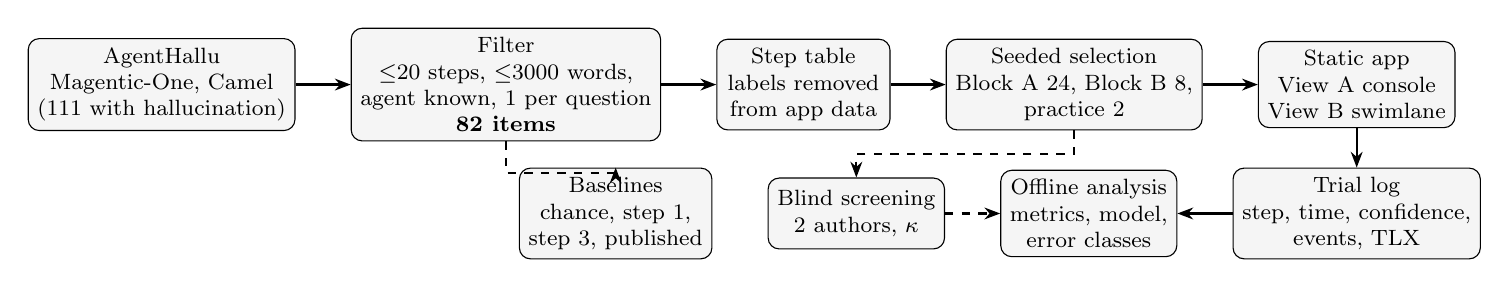
\begin{tikzpicture}[node distance=5mm and 7mm, every node/.style={font=\footnotesize},
box/.style={draw, rounded corners, align=center, minimum height=9mm, minimum width=22mm, fill=gray!8},
arr/.style={-{Stealth[length=2mm]}, thick}]
\node[box] (data) {AgentHallu\\Magentic-One, Camel\\(111 with hallucination)};
\node[box, right=of data] (pool) {Filter\\$\le$20 steps, $\le$3000 words,\\agent known, 1 per question\\\textbf{82 items}};
\node[box, right=of pool] (table) {Step table\\labels removed\\from app data};
\node[box, right=of table] (sel) {Seeded selection\\Block A 24, Block B 8,\\practice 2};
\node[box, right=of sel] (app) {Static app\\View A console\\View B swimlane};
\node[box, below=of app] (log) {Trial log\\step, time, confidence,\\events, TLX};
\node[box, left=of log] (an) {Offline analysis\\metrics, model,\\error classes};
\node[box, left=of an] (scr) {Blind screening\\2 authors, $\kappa$};
\node[box, left=of scr] (base) {Baselines\\chance, step 1,\\step 3, published};
\draw[arr] (data)--(pool); \draw[arr] (pool)--(table); \draw[arr] (table)--(sel); \draw[arr] (sel)--(app);
\draw[arr] (app)--(log); \draw[arr] (log)--(an); \draw[arr,dashed] (scr)--(an);
\draw[arr,dashed] (sel.south) |- ($(sel.south)+(0,-3mm)$) -| (scr.north);
\draw[arr,dashed] (pool.south) |- ($(pool.south)+(0,-4mm)$) -| (base.north);
\end{tikzpicture}
\caption{Study pipeline. Solid arrows: implemented and run. The trial log was produced only by the two authors' sessions; analysis of classmate data was not run because none exists. Dashed arrows: participant-free checks (baselines, blind screening).}
\label{fig:arch}
\end{figure*}

\subsection{The two views}
View A is one scrolling column with each step headed ``[Step $k$] Agent'', a find box with highlights, match count and next/previous, and a ``Select this step'' button per step. View B is an SVG swimlane with one row per agent and steps left to right, mark fill for message versus tool call (two colour-blind-safe hues), an arrow between consecutive steps when the speaker changes, the same find box with matches ringed on the lanes, and a panel with the full text of the selected step. In both views tool output over 150 words sits behind an ``Expand'' control, and the answer action and confirmation are identical. Views are labelled ``View A'' and ``View B'' so that neither is presented as new. View B adds only derived marks (lane position, mark shape and colour, arrows, rings); it shows no text the console lacks. Block B adds a badge ``AI suggests this step'' with no rationale.

\subsection{Item selection}
\noindent\fbox{\parbox{0.95\columnwidth}{\footnotesize
\textbf{Algorithm 1: item selection (seed 20261113).}\\
1. Build the pool $P$ (82 items); compute the median word count $m$.\\
2. Label each item early ($y\le3$) or later ($y\ge4$), short ($\le m$) or long.\\
3. Block A: draw 6 items per (position, length) cell such that no step number occurs in more than 6 items.\\
4. Block B: 4 early (two at step 1, two at step 3) and 4 later items; each gets a correct and a wrong suggestion, the wrong one being the nearest step at least 2 steps from $y$, preferring a different agent.\\
5. Practice: 2 short early items, not scored.\\
6. Assert all balance constraints; write the item set and hash.}}

\subsection{Changes after the Phase 2 feedback}
The class feedback on the Phase 2 design is already reflected in the design document, which we treat as the current plan. Changes made while implementing it are in Table~\ref{tab:dev} and each is logged with date and impact in the project's decision log.

\begin{table}[t]
\centering\footnotesize
\caption{Deviations from the planned design and their effect on claims.}
\label{tab:dev}
\begin{tabular}{@{}p{0.5cm}p{3.7cm}p{3.5cm}@{}}
\toprule
\# & Change & Effect\\
\midrule
D1 & LLM baseline skipped; published 41.1\% cited & Human-versus-LLM question unanswerable\\
D2 & Wrong suggestions rule-based, not LLM errors & Weakens the suggestion hypothesis\\
D3 & Block A labels never shipped in app & None\\
D8 & Team-member sessions labelled PILOT & Descriptive only\\
D10 & 23 items flagged in screening kept & Weakens label-validity claims\\
D9 & Model fallback order fixed in advance & Intervals are posterior, may be narrow\\
\bottomrule
\end{tabular}
\end{table}

%% ------------------------------------------------------------------
\section{Experimental Setup}\label{sec:setup}
\textbf{Data.} AgentHallu \cite{liu2026agenthallu}, commit 9ffe8bc (Magentic-One and Camel subsets). The repository states CC BY 4.0 and the paper CC BY-NC-SA 4.0; we follow the stricter terms. The data folder was treated as untrusted: scripts read it with isolated Python and the \texttt{.env} file was not opened. Filters reduce 111 hallucinating trajectories to 104 (at most 20 steps), 83 (at most 3,000 words), 82 (responsible agent known; one trajectory per question). The pool reproduces every number planned: 47 Magentic-One and 35 Camel items, 46 labels at step 3, median length 1,135.5 words, and 6 later-position items below the median.

\textbf{Splits.} Nothing is trained, so there is no train/test split. The counterbalancing takes its place: Block A's 24 items form two halves of 12, each split into two sets of 6 (3 early, 3 later, 3 short, 3 long); four lists and two view orders give 8 cells, and participant $n$ takes cell $(n-1)\bmod 8$.

\textbf{Study protocol (not run).} Within-subjects; Block A 12 trials, 6 per view; Block B 4 trials with suggestions; 4-minute cap per trial; raw NASA-TLX after each view block; target $N=32$, minimum 24. A planning simulation (assumed variances 0.8 and 1.0 logit; a hypothetical 40\% baseline) gives power 0.51, 0.62, 0.74 for a 15-point gain at $N=24,32,40$ and 0.75, 0.86, 0.93 for 20 points. These are assumptions, not results.

\textbf{Baselines.} Chance, ``always step 1'' and ``always step 3'' on the final item set, and the published best LLM figure (not item-matched). No LLM was called (Section~\ref{sec:disc}).

\textbf{Metrics.} Section~III-A, plus Cohen's $\kappa$ \cite{cohen1960kappa} for screening agreement and agreement within one step.

\textbf{Screening.} Both authors labelled the first hallucinated step blind, in the console view, for the 32 scored items, the 2 practice items and 11 reserves. Practice items are excluded from agreement because their labels had been shown as feedback.

\textbf{Implementation and environment.} Static HTML, CSS, JavaScript and SVG, no network calls; Python 3.15.0, NumPy 2.5.4, SciPy 1.18.1, pandas 3.0.6, statsmodels 0.15.0, Matplotlib 3.11.2 on Windows 11. Hardware (CPU, memory) was not recorded; nothing in the work is compute-heavy. Seeds: item selection 20261113, suggestion key 20261114, screening order 20261114, reserves order 20261115, power simulations 7 and 20261113, bootstrap 20261201. All are in \texttt{results/run\_info.json}. Code and outputs are in the public repository \url{https://github.com/abdullahwaheed0112/hallucination-attribution-study}.

%% ------------------------------------------------------------------
\section{Results and Analysis}\label{sec:results}
\textbf{Item set.} The final set has 24 Block A items (16 Magentic-One, 8 Camel; 6 per position-by-length cell), 8 Block B items, 2 practice items and 11 reserves. The later-position stratum is used up: of 17 later items, Block A takes 12 (all 6 short ones), Block B 4 and 1 remains. Fig.~\ref{fig:f2} shows the balance.

\textbf{Baselines.} Table~\ref{tab:base} gives the computed values (exact / agent / tolerant, \%).

\begin{table}[t]
\centering\footnotesize
\caption{Baseline accuracy (\%), computed from the data; exact / agent / tolerant ($\pm1$ step). *Published figure, not item-matched.}
\label{tab:base}
\begin{tabular}{@{}lcccc@{}}
\toprule
Set & $n$ & Chance & Step 1 & Step 3\\
\midrule
Pool & 82 & 16.5/50.9/43.5 & 22.0/29.3/23.2 & 56.1/69.5/62.2\\
Block A & 24 & 16.3/56.1/39.5 & 25.0/41.7/29.2 & 20.8/54.2/37.5\\
Block B & 8 & 12.2/45.4/34.3 & 25.0/37.5/25.0 & 25.0/62.5/37.5\\
Selected & 34 & 15.3/51.7/38.3 & 26.5/41.2/29.4 & 23.5/55.9/38.2\\
\midrule
\multicolumn{5}{@{}l}{Published best LLM (Gemini-2.5-Pro), exact: 41.1*}\\
\bottomrule
\end{tabular}
\end{table}

\emph{Data show.} On the pool, always step 3 scores 56.1\%, more than three times chance (16.5\%), because 46 of 82 labels sit at step 3. On Block A both position rules score 20.8--25.0\%. Inside Block A's early stratum (12 items) always step 1 scores 50.0\% and always step 3 41.7\%; in the later stratum both score 0\% (Fig.~\ref{fig:f1}). \emph{Interpretation.} Balancing removes the shortcut for the set as a whole but not within the early stratum, where half the items are step-1 items. Fig.~\ref{fig:f3} adds that chance accuracy falls with trace length: long traces are harder to hit by guessing, so length and position must also be read together. Position strata must therefore be analysed together with any view effect. \emph{Conclusion.} The item set meets its balance targets at the set level; a high accuracy on early items alone cannot be credited to a view.

\begin{figure}[t]
\centering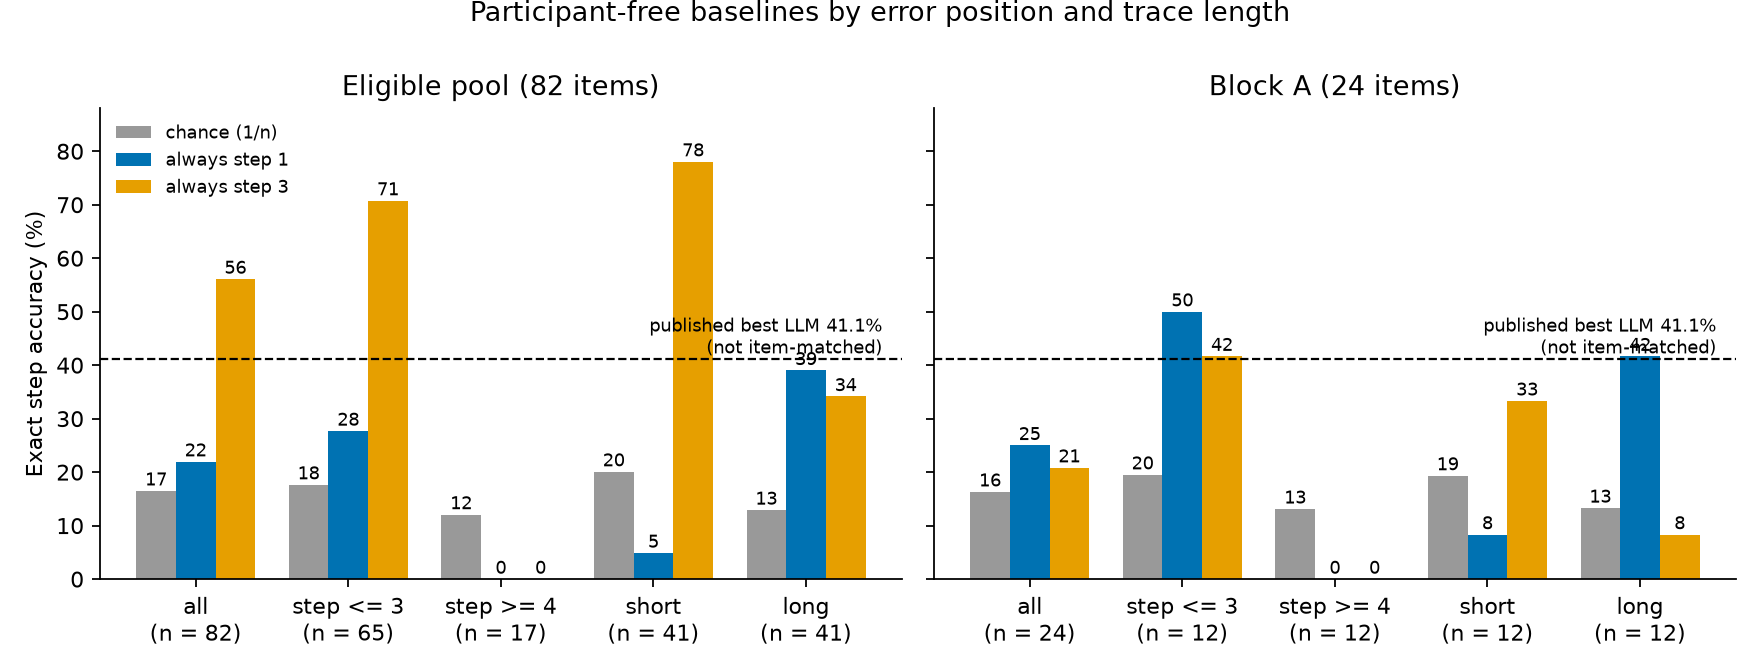
\includegraphics[width=\columnwidth]{F1_baseline_accuracy_by_strata.png}
\caption{Exact accuracy of the baselines by position and length strata, pool and Block A. The published 41.1\% is marked as not item-matched. No participant data.}
\label{fig:f1}
\end{figure}

\begin{figure}[t]
\centering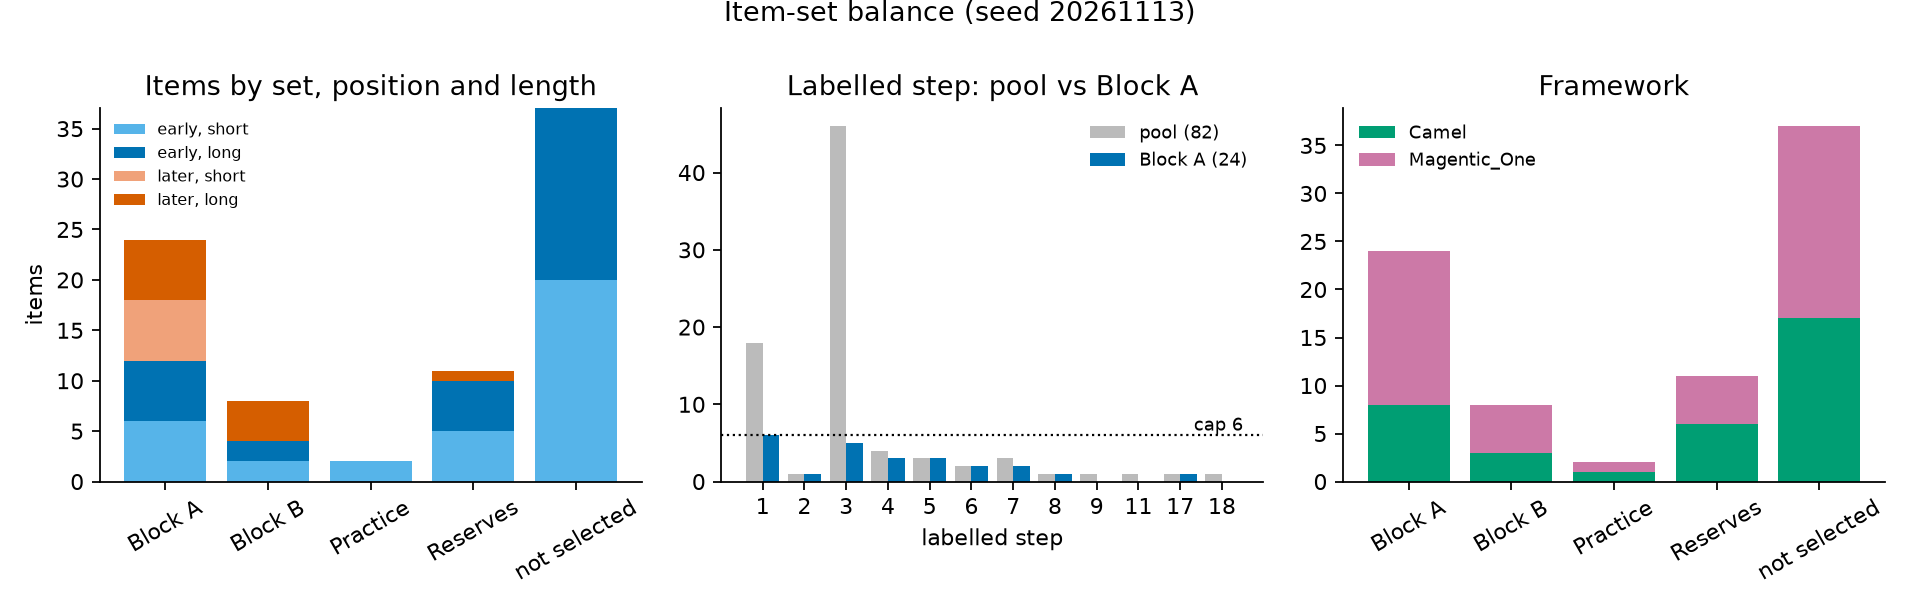
\includegraphics[width=\columnwidth]{F2_item_set_balance.png}
\caption{Item-set balance: items by set, position and length; labelled-step counts against the cap of 6; framework by set.}
\label{fig:f2}
\end{figure}

\begin{figure}[t]
\centering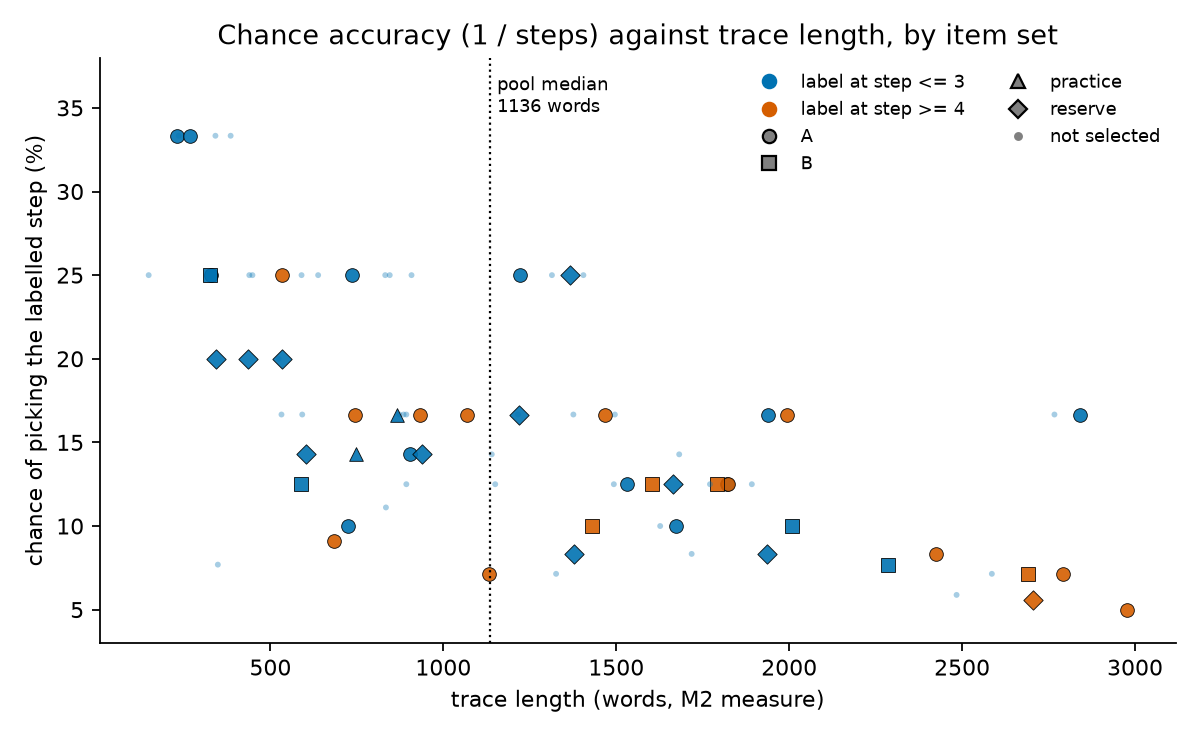
\includegraphics[width=\columnwidth]{F3_item_difficulty_chance.png}
\caption{Chance accuracy ($1/n$ steps) against trace length by item set. In the pool, words and $1/n$ steps correlate at $-0.64$.}
\label{fig:f3}
\end{figure}

\textbf{Label validity (screening).} Table~\ref{tab:screen} reports the two authors' blind screening.

\begin{table}[t]
\centering\footnotesize
\caption{Blind screening on the 32 scored items (AW, AM: the two authors).}
\label{tab:screen}
\begin{tabular}{@{}lc@{}}
\toprule
Measure & Value\\
\midrule
Cohen's $\kappa$ (AW vs.\ AM) & 0.261\\
Exact agreement (chance 0.154) & 0.375\\
Agreement within one step & 0.594\\
AW vs.\ label: exact / within one & 0.250 / 0.375\\
AM vs.\ label: exact / within one & 0.125 / 0.281\\
Both differ from label by $>1$ step & 18 of 32\\
Reserves ($n=11$): $\kappa$; both differ & 0.238; 5 of 11\\
Median seconds per item (AW; AM) & 85.8; 119.1\\
\bottomrule
\end{tabular}
\end{table}

\emph{Data show.} The screeners agreed only weakly with each other and rarely reproduced the label; on scored items AW chose a later step than the label 16 times and AM 21 times, an earlier one 7 times each. \emph{Interpretation.} Undergraduates reading for about 1.5--2 minutes per item rarely reproduce the first-step label. The data cannot separate label error from screener error, so we do not claim the labels are wrong; they show that the label is contestable for many items, consistent with the $\alpha=0.64$ step agreement among annotators in a related benchmark \cite{chen2026elephant}. \emph{Conclusion.} Screening does not validate the label set. We kept all 32 scored items (D10) because removing the flagged ones would leave 14; any later human result must be read with tolerant accuracy and a sensitivity analysis excluding flagged items.

\textbf{Pilot (PILOT, one researcher session, descriptive).} Session P01 comprised 6 console and 6 visual Block A trials. Exact matches were 2 of 6 (console) and 1 of 6 (visual), within one step 4 of 6 and 1 of 6; median trial time 75.9\,s and 52.8\,s; raw workload 56.7 and 43.3; confidence was 5 on 17 of 18 trials. The second session (P02, median 4.6\,s per trial) was a click-through that checked the app's flow and logging and is not analysed. These numbers show that the pipeline reads and scores a real export; they are not evidence about either view, because one person who built the app answered different items in each view, and the near-constant confidence makes the Brier score uninformative. No observer notes were taken. No test or interval is reported for the pilot; Fig.~\ref{fig:p1} shows the trials descriptively.

\begin{figure}[t]
\centering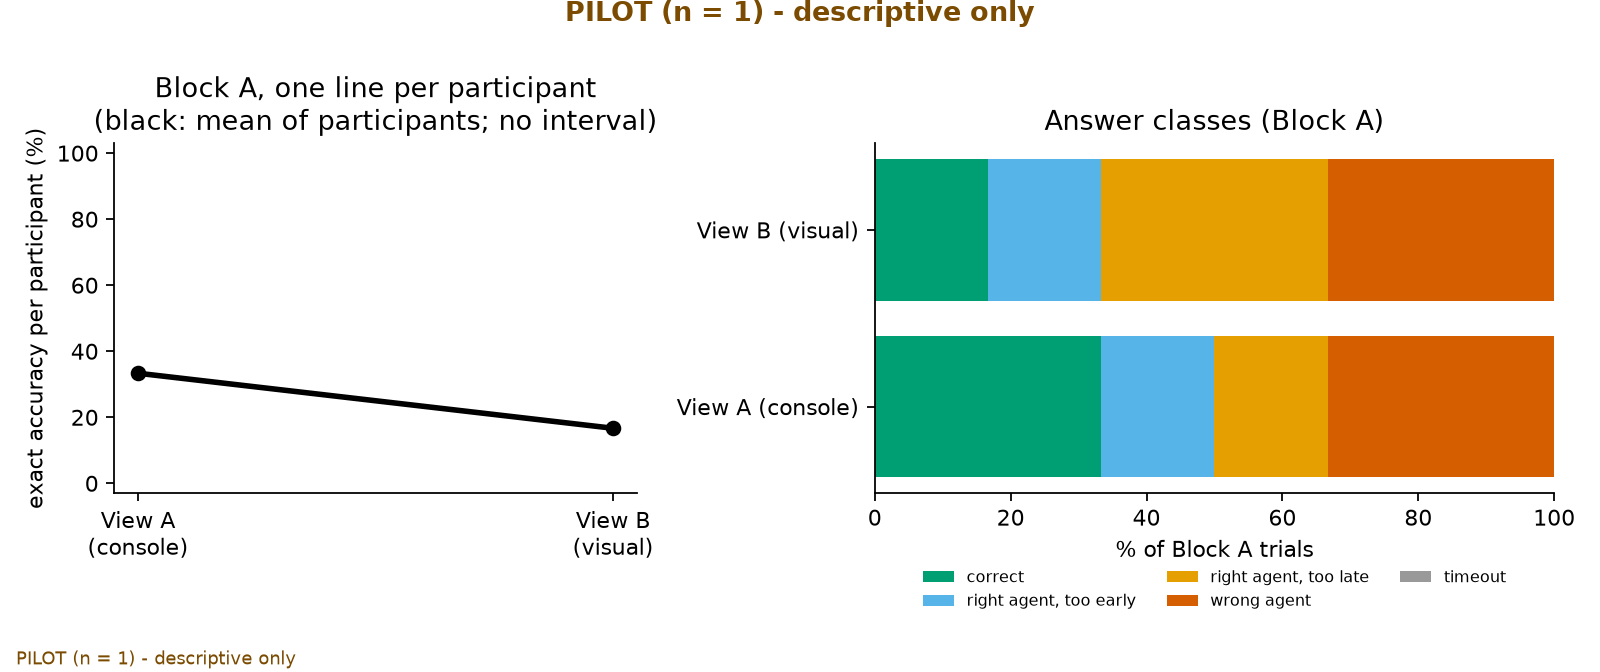
\includegraphics[width=\columnwidth]{P1_pilot_trials_PILOT.png}
\caption{P01 pilot trials, PILOT, descriptive only (one session).}
\label{fig:p1}
\end{figure}

\textbf{Analysis-code testing.} The mixed model and other analysis code were tested on simulated data only; those outputs are labelled SIMULATED in the project and are not findings. A recovery test with a pass rule fixed beforehand passed. At the planned size its intervals covered the injected truth less often than nominal, so intervals from the variational mixed model are posterior intervals that may be too narrow; the paired test and a bootstrap are the robustness checks.

%% ------------------------------------------------------------------
\section{Comparison with Base Papers and State of the Art}
\subsection{Summary of base papers}
Table~\ref{tab:cmp} lists the base papers. Figures come from the papers or from the project's literature notes.

\begin{table*}[t]
\centering\footnotesize
\caption{Base papers. $^\dagger$Version note: the arXiv abstract of TraceElephant reports 30.3\% step and 65.9\% agent accuracy; the figures here are from the PDF we read. Zhou et al.'s arXiv version reports 85.6/82.5/80.6/73.5\%; the IUI PDF we read gives 85.2/80.1/79.3/66.1\%.}
\label{tab:cmp}
\begin{tabular}{@{}p{2.2cm}p{3.1cm}p{2.7cm}p{2.7cm}p{5.3cm}@{}}
\toprule
Paper & Problem and data & Method / metric & Result & Key limitation for comparison\\
\midrule
AgentHallu \cite{liu2026agenthallu} & Hallucination attribution; 693 trajectories, 7 frameworks & 13 LLMs; step localisation & Best 41.1\%; 11.6\% on tool-use & LLMs only; not item-matched to our 82 items\\
TraceElephant \cite{chen2026elephant} & Failure attribution; 220 failed traces & Automated; agent and step accuracy & Step 33.3\%, agent 66.7\%$^\dagger$ & Different label (earliest step after which failure is inevitable); no humans\\
DiLLS \cite{sheng2026dills} & Diagnose failures; Magentic-One on GAIA; 4 cases & Layered summaries vs.\ logs; $N=12$ & Failures found 3.67 vs.\ 2.25 & No ground truth; baseline lacked summaries\\
Zhou et al.\ \cite{zhou2026verification} & Find wrong step in CoT; GSM8K-based; $N=125$ & Interactive formats; accuracy & Graph 85.2\%, plain 66.1\%$^\dagger$ & Single-model maths, not agent turns\\
Kim et al.\ \cite{kim2025reliance} & Factual QA with AI answers; $N=308$ & Explanations, sources; agreement & Agreement with wrong AI 68.2--82.8\% & QA, AI accuracy fixed at 50\%\\
Spatharioti et al.\ \cite{spatharioti2025search} & Car comparison; $N=90$ and 120 & LLM vs.\ web search; accuracy & 47\% vs.\ 93\% on error-prone task & Different models in two experiments\\
\bottomrule
\end{tabular}
\end{table*}

\subsection{Quantitative comparison}
No human result exists in this work, so no accuracy of ours can be set against a base paper's human or LLM accuracy. Table~\ref{tab:quant} shows the only numbers that can sit side by side, each with its provenance.

\begin{table}[t]
\centering\footnotesize
\caption{Exact step accuracy (\%). *Taken from the original paper, not re-implemented or item-matched.}
\label{tab:quant}
\begin{tabular}{@{}p{4.2cm}cp{1.8cm}@{}}
\toprule
Method (data) & Exact & Source\\
\midrule
Chance, pool (82 items) & 16.5 & computed\\
Always step 3, pool & 56.1 & computed\\
Always step 3, Block A & 20.8 & computed\\
Best LLM, AgentHallu (all frameworks) & 41.1* & \cite{liu2026agenthallu}\\
Best method, TraceElephant & 33.3* & \cite{chen2026elephant}\\
Best method, Who\&When hand-crafted & 8.77* & \cite{zhang2025whowhen}\\
Humans, either view & \multicolumn{2}{l}{not measured}\\
\bottomrule
\end{tabular}
\end{table}

\subsection{Methodological comparison and improvement analysis}
Unlike the benchmark papers, we study people, not models. Unlike DiLLS, both views carry the same text, so a difference would be attributable to structure, and answers are scored against labels. Unlike Zhou et al., the object is a multi-agent trace and the encoding is a swimlane, not a dependency graph, because a trace is a sequence of turns by different agents and a graph would require links the data do not contain. Unlike Kim et al.\ and Spatharioti et al., our suggestions are a bare step highlight without rationale.

\textbf{Improvement.} We claim no absolute or relative improvement over any base paper, because we have no human result. One observation needs care: on our pool the trivial rule ``always step 3'' scores 56.1\%, above the published 41.1\% for the best LLM. This is a property of the pool, where 46 of 82 labels are at step 3, and not evidence about LLMs; it is the reason the items were balanced.

\subsection{Fairness and limitations}
The published figures differ in task, label definition, item mix and annotators, and TraceElephant and AgentHallu define the target step differently. We did not re-implement any base method. The 41.1\% covers all frameworks and categories. Zhou et al.\ reached high accuracy partly because most of their items contain errors, so a constant answer scores high. Where our method cannot outperform a base paper, there is nothing to report, as we have no human measurement.

%% ------------------------------------------------------------------
\section{Ablation Study}\label{sec:ablation}
All ablations are participant-free and LLM-free; definitions were written before they were run. \textbf{The ablation of the view components (lane marks, arrows, search marks, details panel) needs participants and is future work.}

\textbf{E1: item features (82 pool items, descriptive).} Category almost fixes the labelled step: all 22 Human-Interaction items (all Camel) are at step 3; 18 of 21 Planning items at step 1; of the 17 items at step 4 or later, 16 are Reasoning. Adjusted $R^2$ of a linear probability model with category alone is 0.81 for ``step 1 hits'' and 0.43 for ``step 3 hits''; position alone gives 0.33 for step 3. \emph{Interpretation.} Position and category are confounded, so their shares cannot be separated, and the outcomes are partly definitional. \emph{Conclusion.} A future finding such as ``accuracy is lower at later positions'' is a statement about this pool's mix of Reasoning hallucinations, not about position alone.

\textbf{E2: representation, without an LLM.} Rule R1 uses the console format (step numbers, agent names); R2 is plain text. Table~\ref{tab:e2} gives exact accuracy of simple rules.

\begin{table}[t]
\centering\footnotesize
\caption{Simple rules on text formats, exact accuracy (\%); rules, not people.}
\label{tab:e2}
\begin{tabular}{@{}lcc@{}}
\toprule
Rule (needs) & Pool & Block A\\
\midrule
Always step 3 (step numbers) & 56.1 & 20.8\\
First non-coordinating agent (agent names) & 57.3 & 25.0\\
First step with tool output (text only) & 36.6 & 8.3\\
First step with a number not in question (text only) & 18.3 & 16.7\\
\bottomrule
\end{tabular}
\end{table}

In plain text 35 of 82 labelled steps (42.7\%) have an empty message, i.e.\ are tool-only steps, and 4 of 82 lose a speaker change. \emph{Interpretation.} Agent names carry as much shortcut value as step numbers in the pool, so the tagged console format offers a shortcut plain text would not; balancing removes it for Block A. \emph{Conclusion.} No rule using agent names or step numbers exceeds 25\% on scored items. This says nothing about how people read either view and does not test the report that step indices raised an LLM's step accuracy \cite{ma2026dover}.

\textbf{E3: component use (P01 only).} In 6 visual-view trials P01 opened more than one step per trial and never used search or the agent filter. With one person and no variation there is nothing to compare, so no association with accuracy can be examined.

%% ------------------------------------------------------------------
\section{Discussion}\label{sec:disc}
\textbf{What the evidence supports.} The instrument works end to end and its two views pass a text-equivalence check that was itself mutation-tested (a one-character change in one view made 175 of 6,439 checks fail). The item set removes the step-3 shortcut at the set level, and the label-validity check shows that the ground truth is weaker than assumed.

\textbf{Why the design should work (a rationale, not a finding).} Lane position makes the agent of each step visible without reading headers, handoff arrows expose coordination, and linked search shows where a value first appears. Whether any of this raises accuracy is untested.

\textbf{Practical implications.} Any study scoring people against first-step labels should report tolerant accuracy and a sensitivity analysis, balance items against position shortcuts, and keep position and category together in analysis.

\textbf{Failure cases.} The first screening file by one author was a click-through (2--4\,s per item) and was discarded; one pilot session was a click-through; the scripted app test found a real bug (the trial timer was stopped as soon as the screen drew), fixed before the pilot; the first self-test run reported 209 failures caused by a bug in the test.

\textbf{Threats to validity.} (i) No participant data: the pilot is one researcher who built the app and screened the same items. (ii) Label noise: kappa is low and flagged items were kept. (iii) Position and category are confounded. (iv) Only two frameworks and 3--20 steps. (v) Block B's wrong suggestions are rule-based, not real LLM errors, so Block B could not say how people treat real LLM errors. (vi) The 41.1\% is not item-matched. (vii) Model intervals can be narrow. (viii) Opening the app by double-click (\texttt{file://}) was not tested; everything ran through a local server.

\textbf{Why no LLM baseline.} No LLM was available in the working environment, so the item-matched baseline was skipped (D1) rather than approximated. The human-versus-LLM question is unanswered.

\textbf{Were the objectives met?} The implementation, dataset, baseline, ablation and comparison objectives were met within the stated limits. \textbf{The research gap was not addressed:} we cannot say whether the visual view helps, whether suggestions change accuracy, or how position and length moderate this. No null or negative human result exists and none should be inferred.

%% ------------------------------------------------------------------
\section{Conclusion and Future Work}
We built an equal-information console and swimlane instrument, a balanced 34-item set from AgentHallu, participant-free baselines and ablations, and a two-screener label check. The raw pool contains a step-3 shortcut worth 56.1\% that balancing reduces to 20.8--25.0\%, and the first-step label is contestable on many items. Future work: (1) run the classmate study after ethics review (the question has not been answered by the instructor); (2) repeat a pilot with an observer; (3) decide how to treat contested labels (re-adjudicate, replace, or sensitivity-only); (4) run an LLM baseline and replace the rule-based wrong suggestions if an LLM becomes available; (5) run the view-component ablation with participants; (6) repeat the novelty search.

%% ------------------------------------------------------------------
\section*{Declarations and Acknowledgements}
\textbf{Data and code availability.} Traces are from AgentHallu (commit 9ffe8bc, \url{https://github.com/liuxuannan/AgentHallu}), credited under its licence terms. Our code, item set, results and app are in \url{https://github.com/abdullahwaheed0112/hallucination-attribution-study}. The datasets themselves are not redistributed, and answer-key files are not included in the repository.

\textbf{Ethics.} No one outside the two authors used the app, because ethics review for a classmate study is unresolved. The two sessions by the authors are researcher tests.

\textbf{Conflict of interest and funding.} None declared; no external funding.

\textbf{AI-tool usage.} General-purpose AI tools were used to assist with writing the item pipeline, study app, analysis scripts and this manuscript. The authors have reviewed, understood and finalized the pipeline, scripts and results.

%% ------------------------------------------------------------------
\bibliographystyle{IEEEtran}
\bibliography{refs}

%% ------------------------------------------------------------------
\appendices
\section{Reproducibility}
From the project folder with the data folder in place (AgentHallu commit 9ffe8bc): rebuild the pool and check it with \texttt{scripts/pool.py} and \texttt{src/pipeline/build\_pool.py} (expects 82 items, 47/35, step 3 = 46, median 1,135.5, 6); select items with \texttt{select\_items.py}; export app data with \texttt{export\_app\_data.py}; compute baselines with \texttt{scripts/baselines.py}; run ablations with \texttt{ablation\_items.py} and \texttt{ablation\_representation.py}. Serve the app with \texttt{python -m http.server 8765 --directory app} and open \texttt{selftest.html}, which must report PASS with 0 failures in 6,439 checks. Reruns are byte-identical except the variational model fit, which differs in the last digits.

\section{How the study would be run}
Participant code $Pnn$; data label TEST for app runs and PILOT only for the authors' sessions. A session has background questions, two practice trials with feedback, Block A in two view blocks with workload sliders and a break, Block B and final questions; export JSON and CSV. Scoring reads the answer key offline, after screening is finished.

\end{document}
